The FEM panel will present users with a selection of FEM
applications that will take a building model generated by the BIM
application and the EVENT from the event application and perform a
deterministic simulation of structural response. Currently, there is one application
available, OpenSees, and there is no application selection box. That
will be modified in future versions to allow users to provide their own
simulation application. The current OpenSees implementation extends the standard OpenSees executable with a pre- and post-processor to take the BIM and EVENT
files and use OpenSees to simulate the response, and return it in an EDP file.

\begin{figure}[!htbp]
  \centering {
    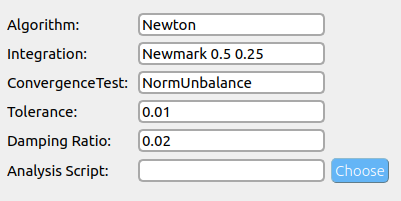
\includegraphics[width=0.5\textwidth]
    {usage/figures/fem.png} }
  \caption{Options for \texttt{OpenSees} transient analysis}
  \label{fig:fem}
\end{figure}

For the OpenSees application the user is required to specify the
options to be used in the transient analysis. As shown in \Cref{fig:fem},
this includes the choice of
\begin{enumerate}
\item \href{http://opensees.berkeley.edu/wiki/index.php/Algorithm_Command}{Solution algorithm}, the default is Newton Raphson.
\item \href{http://opensees.berkeley.edu/wiki/index.php/Integrator_Command}{Integration Scheme}, the default is Newmark's linear acceleration
  method.
\item \href{http://opensees.berkeley.edu/wiki/index.php/Test_Command}{Convergence Test}, the default is a norm on the unbalance force.
\item Convergence tolerance, with a default of 0.01.
\item Damping Ratio. the default is 2\% equivalent viscous damping entered as 0.02. If
a damping ratio of 0 is specified, no damping is added by the simulation application. This allows users to add their own damping in the OpenSees tcl script they load under SIM.
\item Analysis Script. This shall be left blank by default. Advanced users of OpenSees who have their preferred analysis script
and wish to provide their own damping model can provide it here.
\end{enumerate}


The options available for each setting can be found in the OpenSees online user
manual.\\

A default transient analysis script is run with these inputs. It is
built for Version 3.0.0+ of OpenSees and uses a divide and conquer
algorithm to overcome convergence issues. This new algorithm
does not work for every nonlinear problem. The actual analysis command
that is created based on the defaults is the following:

\begin{verbatim}
numberer RCM
system Umfpack
integrator Newmark 0.5 0.25
test NormUnbalance 0.01 20 
algorithm Newton
analysis Transient -numSubLevels 2 -numSubSteps 10 
analyze $numStep $dt
\end{verbatim}

If the user specifies their own analysis script to run
instead of the default, they can take advantage of the \texttt{numStep} and \texttt{dt} variables that
are obtained from the EVENT and are automatically set by the program.